\chapter{Related Work}
\label{ch:RelatedWork}

This chapter presents an overview of existing technologies and research efforts relevant to the development of efficient, on-device language model-based applications. It focuses on three major areas: Retrieval-Augmented Generation (RAG), efficient LLM runtimes like \texttt{llama.cpp}, and lightweight distribution and serving solutions such as Ollama and Llamafile. It also looks at the work done by the tinygrad project in attempting to reverse engineer the NPU API.


%----------------------
\section{RAG Frameworks and Agentic Systems}
\label{sec:RAG}
%----------------------

Retrieval-Augmented Generation (RAG) has become a widely adopted paradigm to enhance the factual grounding of large language models (LLMs) by integrating external knowledge through retrieval mechanisms. To support this architecture, several frameworks have been developed to facilitate the construction of RAG pipelines. \textbf{LangChain}~\cite{langchain} provides a composable and extensible framework for chaining LLMs with retrieval components, supporting a broad ecosystem of vector stores, retrievers, and tools. \textbf{LlamaIndex} (formerly GPT Index)~\cite{llamaindex} offers structured pipelines for indexing and querying private or domain-specific data sources. \textbf{Haystack}~\cite{haystack} by deepset provides a modular toolkit for constructing production-ready pipelines with retriever-reader architectures.

In parallel, the emergence of \textbf{agentic systems}—LLM-powered agents capable of tool use, memory, and reasoning—has opened new avenues for task-oriented automation. Frameworks such as LangChain~\cite{langchain} and AutoGen~\cite{autogen} support multi-agent orchestration and planning. These systems increasingly incorporate \textbf{LLM routing} strategies~\cite{gor2023router} that dynamically select or combine multiple models or tools based on the query or context, enhancing efficiency and specialization. Additionally, \textbf{RAGAS}~\cite{ragas} introduces an evaluation framework to measure the quality and factual alignment of RAG outputs, contributing to the robustness of such systems in real-world applications. Together, these frameworks and methodologies form the foundational ecosystem for deploying scalable, intelligent, and grounded LLM applications.

Although this project does not directly leverage any existing RAG frameworks yet, it certainly has drawn inspiration and insights wherever applicable.

%----------------------
\section{llama.cpp}
\label{sec:llama_cpp}
%----------------------

\texttt{llama.cpp}\cite{gerganov2020llamacpp} is a C++ implementation of large language models (Meta LLaMA to begin with), optimized for local inference on commodity hardware without GPU requirements. Built upon the GGML tensor library, it provides quantized inference for large models using CPU-friendly formats like 4-bit or 5-bit quantization, making it suitable for running models such as LLaMA, Mistral, and other open-weight transformers on devices ranging from laptop to Raspberry Pi.

Key features of \texttt{llama.cpp} include:
\begin{itemize}
    \item Highly efficient CPU inference with quantized models.
    \item Cross-platform support (macOS, Linux, Windows).
    % \item Integration with popular tooling such as LangChain and Open Interpreter.
    \item Support for multi-threaded inference and memory-mapped model weights for efficient memory usage.
\end{itemize}

Llama.cpp serves as a foundational component for many desktop LLM applications that prioritize local execution and privacy-preserving computation. \textit{In this project (Project TLDR), llama.cpp is used for LLM inference tasks, including both embedding generation and text generation}.

%----------------------
\section{Ollama}
\label{sec:ollama}
%----------------------

Ollama is a developer-friendly platform for running LLMs locally with simplified model management and serving. It wraps models like LLaMA 2, Mistral, and Code LLaMA into a streamlined runtime with a CLI and RESTful API, abstracting away hardware-specific setup and providing a plug-and-play experience for developers \cite{ollama}.

Ollama supports:
\begin{itemize}
    \item Running quantized models locally with GPU acceleration where available.
    \item Seamless model downloading and serving.
    % \item Custom model creation using a simple Modelfile syntax.
\end{itemize}

It is widely used for prototyping private, offline chatbots and assistants. However, the users need to be technically savvy in cases of issues downloading or running the models. Furthermore, models often may not be quantized and could lead to downloading of model weights in order of many GBs.


%----------------------
\section{Llamafile}
\label{sec:llamafile}
%----------------------


Llamafile, developed by Mozilla-Ocho, enables packaging a complete LLM runtime into a single, self-contained executable file \cite{llamafile}. It leverages the \texttt{llama.cpp} backend and Cosmopolitan Libc to build universal binaries that run across major operating systems (Windows, macOS, Linux) without requiring dependencies.

Notable features:
\begin{itemize}
    \item Distributable as a single file.
    \item Useful for shipping LLM-based tools with zero-install requirements.
    \item Integrates with web frontends for local chatbot deployment.
\end{itemize}

Llamafile is widely used for prototyping private, offline chatbots and assistants. However, it often requires users to be technically proficient, especially when encountering issues related to downloading or executing models. Moreover, many models are not pre-quantized, potentially resulting in downloads of several gigabytes of model weights.
%----------------------
\section{Tinygrad project and Apple Neural Engine (ANE)}
\label{sec:ANEAPI}
%----------------------

The Apple Neural Engine (ANE) is a custom neural processing unit designed by Apple to accelerate machine learning workloads on its silicon platforms. Introduced with the A11 Bionic chip, the ANE has evolved into a high-performance, low-power DMA-based inference engine embedded in Apple's M-series chips. This section synthesizes insights obtained by the reverse-engineering efforts of the \texttt{tinygrad}~\cite{tinygrad2023ane} project to examine ANE's architecture, capabilities, and compilation flow.

\subsection{Hardware Overview}

The ANE operates primarily as a DMA engine optimized for convolutional operations and supports a wide range of neural network layers and fused operations. Its key hardware features include:

\begin{itemize}
  \item \textbf{16-core architecture:} A 16-wide Kernel DMA engine for parallel computation.
  \item \textbf{5D Tensor Support:} Tensors are structured with width (column), height (row), planes (channels), depth, and group (batch).
  \item \textbf{Supported Data Types:} \texttt{UInt8}, \texttt{Int8}, and \texttt{Float16} (with \texttt{Float32} inputs automatically downcast).
  \item \textbf{Manually Managed 4MB L2 Cache:} Applied only to input/output data; weights are embedded in the compiled program.
  \item \textbf{Execution Unit:} Executes up to 0x300 micro-operations per instruction.
  \item \textbf{Performance:} Approximate 11 TOPS throughput, assuming 32\texttimes32 MAC at ~335 MHz.
\end{itemize}

All memory strides are constrained to multiples of 0x40 bytes, reflecting hardware alignment requirements.

\subsection{Software and Compilation Stack}

The ANE software stack is heavily abstracted behind Apple's proprietary frameworks but has been reverse-engineered to reveal a structured flow (as shown in Fig~\ref{fig:ane-workflow}):
\begin{figure}[h]
    \centering
    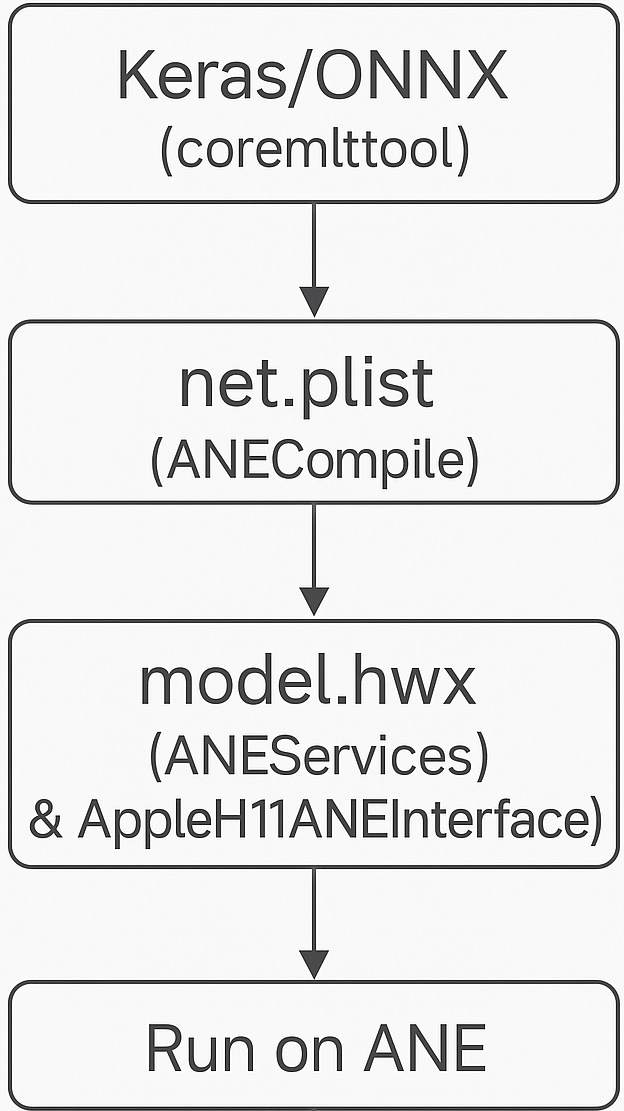
\includegraphics[width=0.25\linewidth]{images/ane-workflow.jpg}
    \caption{Apple Neural Engine Workflow}
    \label{fig:ane-workflow}
\end{figure}

\begin{enumerate}
  \item \textbf{Model Definition:} Models are authored in Keras or ONNX.
  \item \textbf{Conversion:} Models are converted to CoreML format using open-source tools such as \texttt{coremltools}.
  \item \textbf{Intermediate Representation:} CoreML is internally converted into \texttt{net.plist} by Apple's Espresso framework.
  \item \textbf{Compilation:} The \texttt{ANECompiler} service transforms \texttt{net.plist} into a hardware-specific binary (.\texttt{hwx}), a Mach-O formatted executable.
  \item \textbf{Execution:} The \texttt{AppleNeuralEngine} and \texttt{ANEServices} handle execution via the kernel extension \texttt{AppleH11ANEInterface}.
\end{enumerate}


\subsection{Instruction Format and Operation Structure}

Each ANE instruction is 0x300 bytes and comprises multiple segments:

\begin{itemize}
  \item \textbf{Header:} Includes DMA addresses and next-op offset.
  \item \textbf{KernelDMASrc:} Specifies weights, bias, and channel usage.
  \item \textbf{Common:} Describes input/output shapes, types, kernel size, and padding.
  \item \textbf{TileDMASrc/TDMADst:} Layout and stride configurations for input/output tensors.
  \item \textbf{L2 and NE:} L2 cache flags and activation parameters.
\end{itemize}

\subsection{Supported Operations and Activations}

ANE supports a variety of operations:

\begin{itemize}
  \item \textbf{Core Ops:} CONV, POOL, EW, CONCAT, RESHAPE, MATRIX\_MULT, TRANSPOSE
  \item \textbf{Advanced:} SCALE\_BIAS, SOFTMAX, INSTANCE\_NORM, BROADCAST, L2\_NORM
  \item \textbf{Fused Ops:} NEFUSED\_CONV, PEFUSED\_POOL, etc.
  \item \textbf{Activations:} RELU, SIGMOID, TANH, CLAMPED\_RELU, PRELU, LOG2/EXP2, CUSTOM\_LUT
\end{itemize}

% Over 30 activation functions are supported in hardware.

\subsection{tinygrad Implementation}

The \texttt{tinygrad} project interfaces directly with ANE through a three-stage pipeline:

\begin{itemize}
  \item \textbf{1\_build:} Generates CoreML models using \texttt{coremltools}.
  \item \textbf{2\_compile:} Uses Objective-C and Apple's private ANECompiler framework to compile models into HWX binaries.
  \item \textbf{3\_run:} Loads HWX binaries and executes them on ANE using custom Objective-C wrappers around \texttt{AppleH11ANEInterface}.
\end{itemize}

The implementation also includes tools like \texttt{hwx\_parse.py} for disassembling HWX files and visualizing internal ops.

\subsection{Security and Access}

Execution on ANE requires system entitlements that are typically unavailable to third-party applications:

\begin{itemize}
  \item \texttt{com.apple.ane.iokit-user-access}
  \item Workarounds: amfid patching, kernel extension modification, or use of provisioning profiles.
\end{itemize}

\subsection{ANE Takeaways}

The ANE represents a proprietary, highly optimized inference accelerator that is difficult to access and understand due to Apple’s closed ecosystem. Reverse engineering, as demonstrated by \texttt{tinygrad}, reveals a modular, DMA-centric architecture capable of executing complex neural network operations at high throughput and low latency. As Apple continues to iterate on the ANE, deeper access and tooling may unlock broader ML deployment options on Apple hardware.
